\begin{frame}
  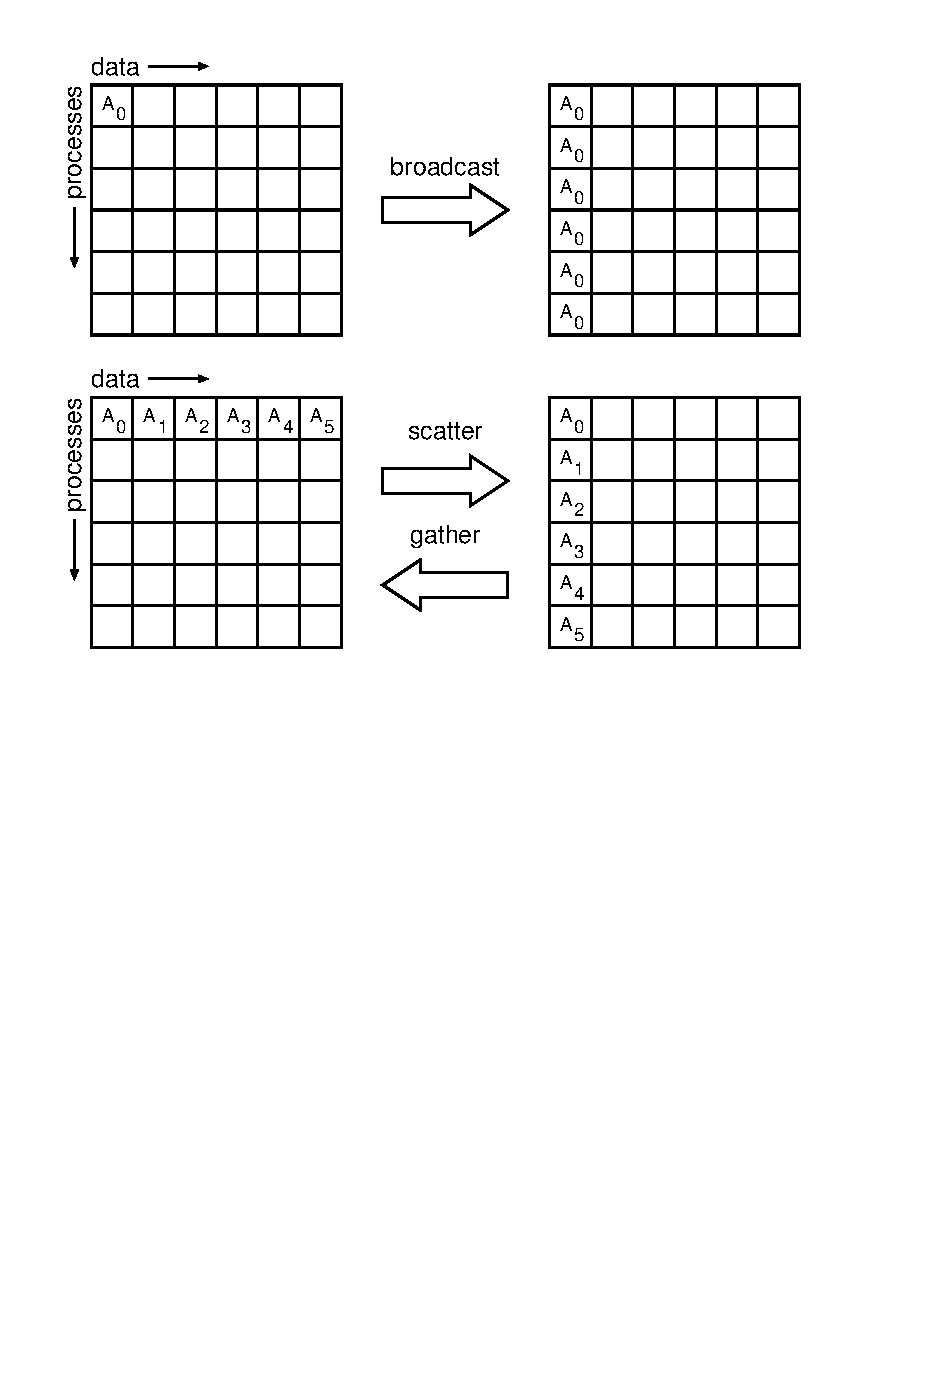
\includegraphics[scale=0.75]{collectives1.pdf}
\end{frame}

\begin{frame}
  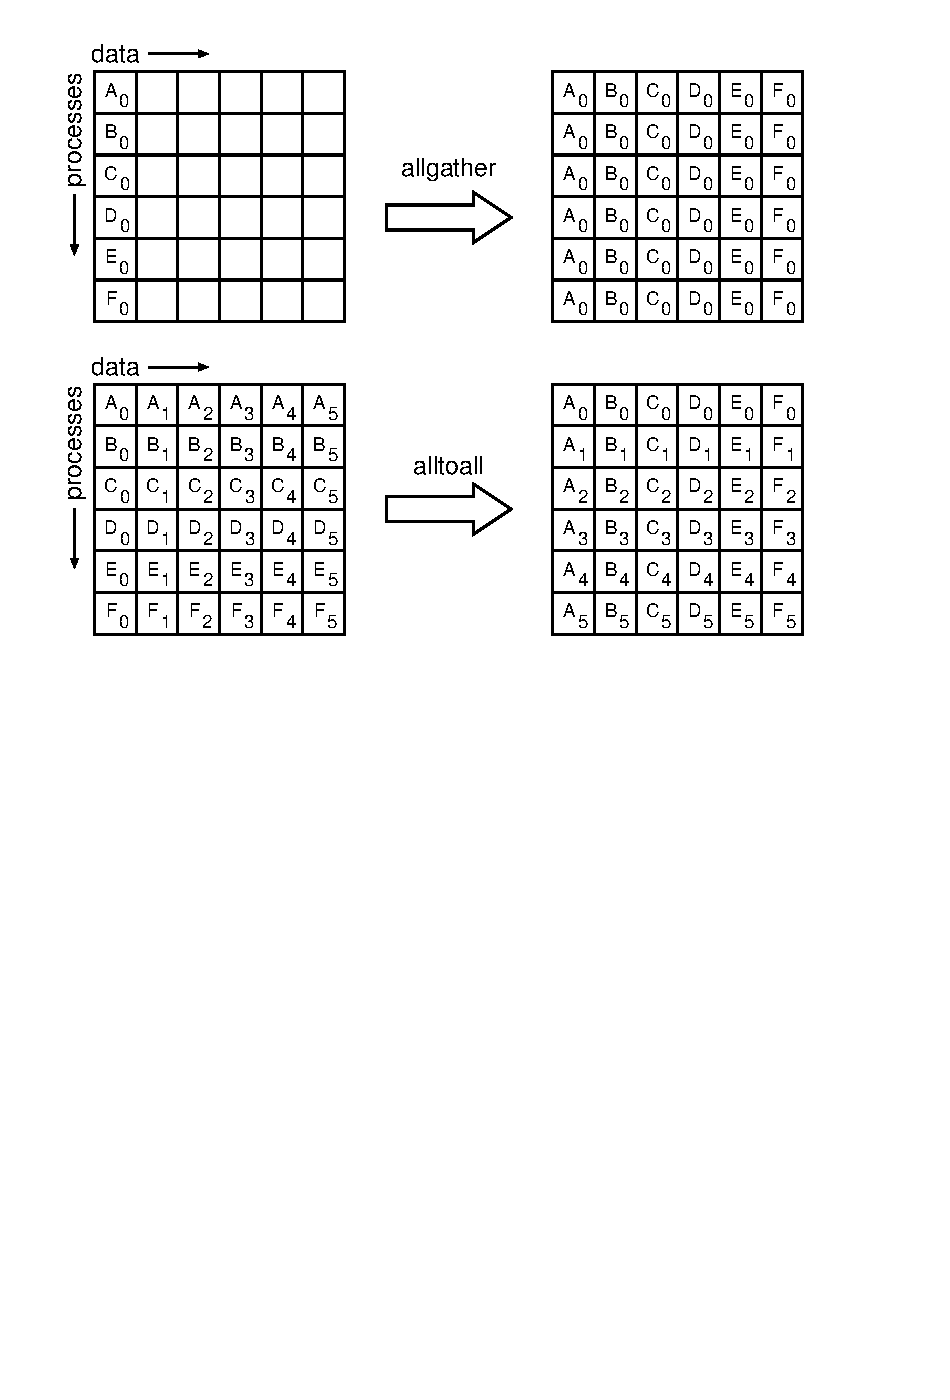
\includegraphics[scale=0.75]{collectives2.pdf}
\end{frame}

\begin{frame}
  \frametitle{Broadcast}
  \inputminted[linenos]{python}{coll_bcast.py}
\end{frame}

\begin{frame}
  \frametitle{Scatter}
  \inputminted[linenos]{python}{coll_scatter.py}
\end{frame}

\begin{frame}
  \frametitle{Gather \& Gather to All}
  \inputminted[linenos]{python}{coll_gather.py}
\end{frame}

\begin{frame}
  \frametitle{Reduce \& Reduce to All}
  \inputminted[linenos]{python}{coll_reduce.py}
\end{frame}

\begin{frame}
  \frametitle{Exercise \#3}
  \begin{enumerate}[a)]
  \item Modify the \emph{Broadcast}, \emph{Scatter}, and \emph{Gather}
    examples to communicate NumPy arrays.
  \item Write a routine implementing parallel
    \emph{matrix}--\emph{vector} product
    \texttt{y~=~matvec(comm,A,x)}.
    \begin{itemize}
    \item the global matrix is dense and square.
    \item matrix rows and vector entries have matching block
      distribution.
    \item all processes own the same number of matrix rows.
    \end{itemize}
    \textbf{Tip}: use \texttt{Comm.Allgather()} and \texttt{numpy.dot()}
  \end{enumerate}
\end{frame}

